% -----------------------------------------------
% Template for ISMIR Papers
% 2025 version, based on previous ISMIR templates

% Requirements :
% * 6+n page length maximum
% * 10MB maximum file size
% * Copyright note must appear in the bottom left corner of first page
% * Clearer statement about citing own work in anonymized submission
% (see conference website for additional details)
% -----------------------------------------------

\documentclass{article}
\usepackage[T1]{fontenc}
\usepackage[utf8]{inputenc}
\usepackage[submission]{ismir} % Remove the "submission" option for camera-ready version
\usepackage{amsmath,cite,url}
\usepackage{graphicx}
\usepackage{color}

% Title. Please use IEEE-compliant title case when specifying the title here,
% as it has implications for the copyright notice
% ------
\title{Violin's Signature: Leveraging Audio Features and Machine Learning for Violin Fingerprinting}

% Note: Please do NOT use \thanks or a \footnote in any of the author markup

% Single address
% To use with only one author or several with the same address
% ---------------
% \oneauthor
%   {Anonymous Authors}
%   {Anonymous Affiliations\\\texttt{anonymous@ismir.net}}

% Two addresses
% --------------
%\twoauthors
%   {First author} {School \\ Department}
%   {Second author} {Company \\ Address}

% Three addresses
% --------------
\threeauthors
  {Hugo Pauget Ballesteros} {Institut d'Alembert \\ {\tt hugo.pauget@dalembert.upmc.fr}}
  {Philippe Lalitte} {IReMus \\ {\tt philippe.lalitte@upmc.fr}}
  {Claudia Fritz} {Institut d'Alembert \\ {\tt fritz@lam.jussieu.fr}}

% Four or more addresses
% OR alternative format for large number of co-authors
% ------------
% \multauthor
%   {First author$^1$ \hspace{1cm} Second author$^1$ \hspace{1cm} Third author$^2$}
%   {{\bf Fourth author$^3$ \hspace{1cm} Fifth author$^2$ \hspace{1cm} Sixth author$^1$}\\
%   $^1$ Department of Computer Science, University, Country\\
%   $^2$ International Laboratories, City, Country\\
%   $^3$ Company, Address\\
%   {\tt\small CorrespondenceAuthor@ismir.edu, PossibleOtherAuthor@ismir.edu}
%   }

% For the author list in the Creative Common license, please enter author names.
% Please abbreviate the first names of authors and add 'and' between the second to last and last authors.
\def\authorname{H. Pauget Ballesteros, P. Lalitte, and C. Fritz}

% Optional: To use hyperref, uncomment the following.
% \usepackage[bookmarks=false,pdfauthor={\authorname},pdfsubject={\pdfsubject},hidelinks]{hyperref}
% Mind the bookmarks=false option; bookmarks are incompatible with ismir.sty.

\sloppy % please retain sloppy command for improved formatting

\begin{document}

\maketitle

\begin{abstract}
Identifying individual instruments of the same type from their recordings is a rarely addressed challenge. This paper explores violin sound identification using two datasets of recordings, featuring multiple violinists playing multiple violins. Several long-term audio features were compared, and their performance in violin classification was evaluated using classical machine learning algorithms. Among these features, long-term MFCCs demonstrated the ability to distinguish individual violins, even with player-induced variability, enabling reliable violin recognition. Additionally, the influence of key parameters—such as the number of violinists and choice of musical excerpts—on classification performance was analyzed. These findings offer guidelines for optimizing future data collection aimed at capturing a violin's unique sound signature.
\end{abstract}

\section{Introduction}\label{sec:introduction}

\section{Methods}\label{sec:methodology}

\subsection{Dataset}
In 2024, a dataset was created at the Paris Conservatoire (CNSMDP), involving thirteen violinists and three violins. The participants were invited to freely explore each instrument before recording a chromatic scale and selected excerpts from the classical violin repertoire. The excerpts included pieces by Bach (Allemande), Mozart (Concerto No. 3), Tchaikovsky (Concerto), Sibelius (Concerto), and Glazunov (Concerto). All recordings were conducted under consistent conditions in a large recording studio at the CNSM. The distance between the performer and the microphone (a pair of DPA 4006) was kept constant, and a sample rate of 48 kHz was used throughout the sessions.

\subsection{Audio features}

\subsubsection{Long Time Average Spectra (LTAS)}

\section{Page Size}\label{sec:page_size}

The proceedings will be printed on \underline{portrait A4-size paper} \underline{(21.0cm x 29.7cm)}. All material on each page should fit within a rectangle of 17.2cm x 25.2cm, centered on the page, beginning 2.0cm from the top of the page and ending with 2.5cm from the bottom. The left and right margins should be 1.9cm. The text should be in two 8.2cm columns with a 0.8cm gutter. All text must be in a two-column format. Text must be fully justified.

\section{Typeset Text}\label{sec:typeset_text}

\subsection{Normal or Body Text}\label{subsec:body}

Please use a 10pt (point) Times font. Sans-serif or non-proportional fonts can be used only for special purposes, such as distinguishing source code text.

The first paragraph in each section should not be indented, but all other paragraphs should be.

\subsection{Title and Authors}

The title is 14pt Times, bold, caps, upper case, centered. \textbf{Authors' names are omitted when submitting for double-blind reviewing.}

\subsection{First Page Copyright Notice}

Please include the copyright notice exactly as it appears here in the lower left-hand corner of the page. It is set in 8pt Times.


\subsection{Page Numbering, Headers and Footers}

Do not include headers, footers or page numbers in your submission. These will be added when the publications are assembled.

\subsection{Line Numbers}

\textbf{Line numbers should be included in your submitted manuscript,} for reference during reviewing.

\section{First Level Headings}

First-level headings are in Times 10pt bold, centered with 1 line of space above the section head, and 1/2 space below it. For a section header immediately followed by a subsection header, the space should be merged.

\subsection{Second Level Headings}

Second-level headings are in Times 10pt bold, flush left, with 1 line of space above the section head, and 1/2 space below it. The first letter of each significant word is capitalized.

\subsubsection{Third and Further Level Headings}

Third-level headings are in Times 10pt italic, flush left, with 1/2 line of space above the section head, and 1/2 space below it. The first letter of each significant word is capitalized. Using more than three levels of headings is highly discouraged.

\section{Footnotes and Figures}

\subsection{Footnotes}

Indicate footnotes with a number in the text.\footnote{This is a footnote.} Use 8pt type for footnotes. Place the footnotes at the bottom of the page on which they appear. Precede the footnote with a 0.5pt horizontal rule.

\subsection{Figures, Tables and Captions}

All artwork must be centered, neat, clean, and legible. All lines should be very dark for purposes of reproduction and art work should not be hand-drawn. The proceedings are not in color, and therefore all figures must make sense in black-and-white form. \textbf{Figure and table numbers and captions always appear below the figure.} Leave 1 line space between the figure or table and the caption. Each figure or table is numbered consecutively. Captions should be Times 10pt. Place tables/figures in text as close to the reference as possible. References to tables and figures should be capitalized, for example, see \figref{fig:example} and \tabref{tab:example}. Figures and tables may extend across both columns to a maximum width of 17.2cm.

\textbf{To enhance accessibility, we strongly encourage the authors to adopt a color blind friendly color palette when making plots.} For Matplotlib users, the `tableau-colorblind10' and `petroff10' color palettes would be good options, which can be enabled by \texttt{plt.style.use('tableau-colorblind10')} and \texttt{plt.style.use('petroff10')}.

\begin{table}
  \centering
  \begin{tabular}{|l|l|}
    \hline
    String value & Numeric value \\
    \hline
    Hello ISMIR  & \conferenceyear \\
    \hline
  \end{tabular}
  \caption{Table captions should be placed below the table.}
  \label{tab:example}
\end{table}

\begin{figure}
  \centering
  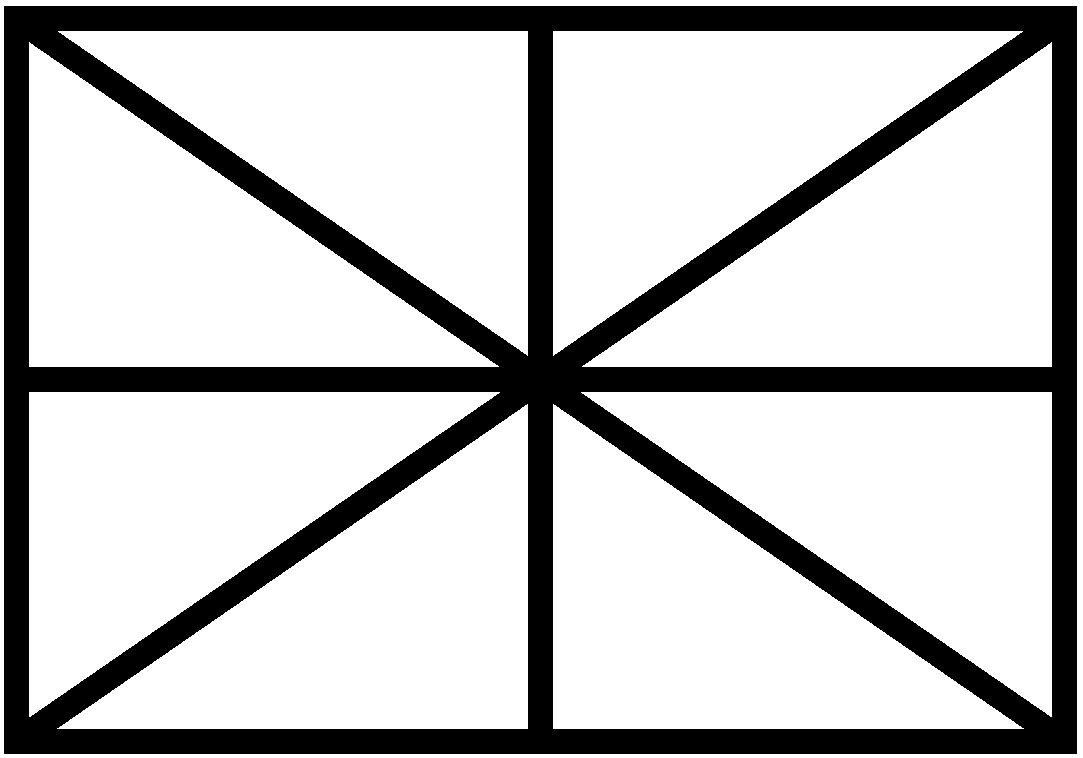
\includegraphics[alt={ISMIR 2025 template example image},width=0.9\linewidth]{example.png}
  \caption{Figure captions should be placed below the figure.}
  \label{fig:example}
\end{figure}

\section{Equations}

Equations should be placed on separate lines and numbered. The number should be on the right side, in parentheses, as in \eqnref{relativity}.

\begin{equation}\label{relativity}
E=mc^{2}
\end{equation}

\section{Citations}

All bibliographical references should be listed at the end of the submission, in a section named ``REFERENCES,'' numbered and in the order that they first appear in the text. Formatting in the REFERENCES section must conform to the IEEE standard (\url{https://ieeeauthorcenter.ieee.org/wp-content/uploads/IEEE-Reference-Guide.pdf}). Approved IEEE abbreviations (Proceedings $\rightarrow$ Proc.) may be used to shorten reference listings. All references listed should be cited in the text. When referring to documents, place the numbers in square brackets (e.g., \cite{ISMIR17Author:01} for a single reference, or \cite{JNMR10Someone:01,Book20Person:01,Chapter09Person:01} for a range).

\textbf{As submission is double blind, refer to your own published work in the third person.} That is, use ``In the previous work of \cite{ISMIR17Author:01},'' not ``In our previous work \cite{ISMIR17Author:01}.'' If you cite your other papers that are not widely available (e.g., a journal paper under review), use anonymous author names in the citation, e.g., an author of the form ``A. Anonymous.''

\section{Acknowledgments}

You may include an optional Acknowledgments section in your camera-ready version to refer to any individuals or organizations that should be acknowledged in your paper. \textbf{Do not include the Acknowledgments section in your submitted manuscript.} The Acknowledgments section does \textit{not} count towards the page limit for scientific content.

\section{Ethics Statement}

You may include an optional Ethics Statement section to provide additional ethical considerations related to your paper. The Ethics Statement section can be included both at submission time and in your camera-ready version. See the Call for Papers for details. The Ethics Statement section does \textit{not} count towards the page limit for scientific content.

\section{Camera Ready Preparation}\label{sec:cameraready}

\textbf{The camera-ready version should include the names, affiliations and email addresses of the authors.} Authors' names are centered. The lead author's name is to be listed first (left-most), and the co-authors' names after. If the addresses for all authors are the same, include the address only once, centered. If the authors have different addresses, put the addresses, evenly spaced, under each authors' name. To display the author information in \LaTeX, please remove the global option `submission' when importing the `ismir' package (i.e., \texttt{\textbackslash usepackage\{ismir\}} in line 16).

\textbf{Please make sure that the author names, paper title and proceedings title are shown correctly in the copyright notice.} For \LaTeX\ users, the proceedings title will be automatically loaded when you remove the global option `submission' when importing the `ismir' package (i.e., \texttt{\textbackslash usepackage\{ismir\}} in line 16). For Word users, you will need to manually replace ``submitted to \textit{ISMIR}, 2025'' to ``in \textit{Proc. of the 26th Int. Society for Music Information Retrieval Conf.}, Daejeon, South Korea, 2025.''

\textbf{You must also remove all line numbers from the final camera-ready version.} This can be done in \LaTeX\ by removing the global option `submission' when importing the ismir package (i.e., \texttt{\textbackslash usepackage\{ismir\}} in line 16). This can be done in Microsoft Word by selecting ``Layout > Line Numbers > None.''

% For BibTeX users:
\bibliography{ISMIRtemplate}

% For non BibTeX users:
%\begin{thebibliography}{citations}
% \bibitem{Author:17}
% E.~Author and B.~Authour, ``The title of the conference paper,'' in {\em Proc.
% of the Int. Society for Music Information Retrieval Conf.}, (Suzhou, China),
% pp.~111--117, 2017.
%
% \bibitem{Someone:10}
% A.~Someone, B.~Someone, and C.~Someone, ``The title of the journal paper,''
%  {\em Journal of New Music Research}, vol.~A, pp.~111--222, September 2010.
%
% \bibitem{Person:20}
% O.~Person, {\em Title of the Book}.
% \newblock Montr\'{e}al, Canada: McGill-Queen's University Press, 2021.
%
% \bibitem{Person:09}
% F.~Person and S.~Person, ``Title of a chapter this book,'' in {\em A Book
% Containing Delightful Chapters} (A.~G. Editor, ed.), pp.~58--102, Tokyo,
% Japan: The Publisher, 2009.
%
%\end{thebibliography}

\end{document}
